\documentclass{beamer}
\usetheme{Madrid}
\usecolortheme{whale}
\usepackage{biblatex}
\addbibresource{similaritybasedcs.bib}
% Customize the color theme
\definecolor{lightblue}{RGB}{70, 70, 255}
\setbeamercolor{structure}{fg=lightblue}
\setbeamercolor{section in toc}{fg=black}
\usepackage{amsmath}
\usepackage[ruled,vlined]{algorithm2e}

% Title Slide
\title{\textbf{Similarity Based Constraint Score}}
\subtitle{Mid-term Research Project Presentation}

\author{Gadegbeku Fabio}
\date{\today}

\begin{document}

% Title Page
\begin{frame}
  \titlepage
  \begin{center}
    \raisebox{-0.5\height}{
\includegraphics[width=0.25\textwidth]{centralelillelogo.png}}\hspace{0.2cm}
    \raisebox{-0.5\height}{
\includegraphics[width=0.25\textwidth]{univlillelogo.png}}\hspace{0.2cm}
    \raisebox{-0.5\height}{
\includegraphics[width=0.25\textwidth]{cristallogo.jpg}}\par
  \end{center}
\end{frame}

% Table Of Contents
\begin{frame}{Table of Contents}
  \tableofcontents
\end{frame}

% Introduction
\section{Introduction}

\begin{frame}{Introduction}
    \begin{block}{Problem : Too many Features}
        \begin{itemize}
            \item Curse of dimensionality
            \item Unnecessarily high computational cost
        \end{itemize}
    \end{block}
\vspace*{1cm}
    \begin{block}{Solution : Feature Selection}
        \begin{itemize}
            \item Tackles the curse of dimensionality
            \item Removes irrelevant or redudant features
        \end{itemize}
    \end{block}
\end{frame}

\begin{frame}{Introduction}
    \begin{block}{Classification Problems}
        \begin{itemize}
            \item We can define \textbf{must link} and \textbf{cannot link} constraints
                \begin{itemize}
                    \item must link : When two samples have the same class
                    \item cannot link : When two samples have different classes
                \end{itemize}
            \item \textbf{Constraint Scores} to evaluate how well each feature respects the constraints
        \end{itemize}
    \end{block}
\end{frame}

\begin{frame}{Introduction}
    \begin{block}{Constraint Scores}
        \begin{itemize}
            \item Typically compute distances between the samples in the original feature space
            \item Still suffer from the curse of dimensionality
        \end{itemize}
    \end{block}
\vspace*{1cm}
    \begin{block}{Solution : Similarity Based Constraint Score (SBCS)}
        \begin{itemize}
            \item Evaluate a whole subset of features at once
            \item Calculates distances in a lower dimensional space
        \end{itemize}
    \end{block}

\end{frame}

\begin{frame}{Introduction}
    \begin{block}{Goals}
        \begin{itemize}
            \item Implement the SBCS as described by \cite{salmiSimilaritybasedConstraintScore2020}
            \item Compare it to other constraint scores on different datasets on multiple criteria
            \item Improve the SBCS by using constraints directly instead of available labels to generate the constraints
        \end{itemize}
    \end{block}
\end{frame}

% Laplacian Score
\section{Laplacian Score}
\begin{frame}{Laplacian Score}
    \begin{block}{Our Data}
     \[ X =
        \begin{bmatrix}
        x_{11} & \dots & x_{1r} & \dots & x_{1d} \\
        \vdots & \ddots & \vdots & \ddots & \vdots \\
        x_{i1} & \dots & x_{ir} & \dots & x_{id} \\
        \vdots & \ddots & \vdots & \ddots & \vdots \\
        x_{n1} & \dots & x_{nr} & \dots & x_{nd} \\
        \end{bmatrix}
        \]
    \end{block}

    \begin{block}{A sample of our Data}
        \[ x_i = (x_{i1}, \dots, x_{ir}, \dots, x_{id})^T \in \mathbb{R}^d \]
    \end{block}

    \begin{block}{A feature vector}
        \[ f_{r} = (x_{1r}, \dots, x_{ir}, \dots, x_{nr})^T \in \mathbb{R}^n \]
    \end{block}
\end{frame}

\begin{frame}{Laplacian Score}

    \begin{block}{Similarity Matrix}
        \[ W = \begin{bmatrix}
            1 & w_{12} & \dots & w_{1n} \\
            w_{21} & 1 & \dots & w_{2n} \\
            \vdots & \vdots & \ddots & \vdots \\
            w_{n1} & w_{n2} & \dots & 1 \\
        \end{bmatrix} \]
    \end{block}

    \begin{block}{Similarity between two samples}
        \[ w_{ij} = S(x_i,x_j) \]
        \\
       For example :  \[ S(x_i,x_j) = \exp(-\frac{||x_i - x_j||^2}{2\sigma^2}) \]
    \end{block}
\end{frame}

\begin{frame}{Laplacian Score}

    \begin{block}{Degree Matrix}
        \[ D = \begin{bmatrix}
            d_{11} & \dots & 0 \\
            \vdots & \ddots & \vdots \\
            0 & \dots & d_{nn} \\
        \end{bmatrix} \]
        \\
        Where : \[ d_{ii} = \sum_{j=1}^n w_{ij} \]
    \end{block}
\end{frame}

\begin{frame}{Laplacian Score}
\begin{block}{Laplacian Matrix}
    \[ L = D - W \]
\end{block}

\begin{block}{Laplacian Score}
    \[
L_r = \frac{\sum_{i=1}^{n} \sum_{j=1}^{n} (x_{ir} - x_{jr})^2 s_{ij}}{\sum_{i=1}^{n} (x_{ir} - \bar{f_{r}}) p_{i}}
\]
\\ Where :  \[ pi = \frac{d_i}{\sum_{k=1}^{n}{d_k}} \]
\\ And we have :
    \[ L_r = \frac{f_r^T L f_r}{f_r^T D f_r} \]
\end{block}
\end{frame}

% Constraint Score 1
\section{Constraint Scores 1 \& 4}
\begin{frame}{Constraint Score 1}
    \begin{block}{Constraints}
        \[
\mathcal{M} = \{(x_i, x_j) \in X \times X \,|\, \text{such that } x_i \text{ and } x_j \text{ are together}\}
\]

\[
\mathcal{C} = \{(x_i, x_j) \in X \times X \,|\, \text{such that } x_i \text{ and } x_j \text{ are not together}\}
\]
    \end{block}

\begin{block}{We can define :}
    \[
w_{ij}^{\mathcal{M}} =
\begin{cases}
  1 & \text{if } (x_i, x_j) \in \mathcal{M} \text{ or } (x_j, x_i) \in \mathcal{M}\\
  0 & \text{else}
\end{cases}
\]
\\

\[
w_{ij}^{\mathcal{C}} =
\begin{cases}
  1 & \text{if } (x_i, x_j) \in \mathcal{C} \text{ or } (x_j, x_i) \in \mathcal{C} \\
  0 & \text{else}
\end{cases}
\]

\end{block}

\end{frame}

\begin{frame}{Constraint Score 1}
    \begin{block}{Minimize}
        \[
\sum_{i=1}^{n} \sum_{j=1}^n (x_{ir} - x_{jr})^2 w_{ij}^{\mathcal{M}}
\]
    \end{block}

    \begin{block}{Maximize}
        \[
\sum_{i=1}^{n} \sum_{j=1}^n (x_{ir} - x_{jr})^2 w_{ij}^{\mathcal{C}}
\]

    \end{block}
\end{frame}

\begin{frame}{Constraint Score 1}
    \begin{block}{New "Laplacian" Matrix}
        \[
L^{\mathcal{M}} = D^{\mathcal{M}} - W^{\mathcal{M}} \quad \text{and} \quad L^{\mathcal{C}} = D^{\mathcal{C}} - C^{\mathcal{C}}
\]
Where :
\[
D_{ii}^{\mathcal{M}} = \sum_{j=1}^n w_{ij}^{\mathcal{M}} \quad D_{ii}^{\mathcal{C}} = \sum_{j=1}^n w_{ij}^{\mathcal{C}}
\]

    \end{block}

    \begin{block}{Constraint Score 1}
        \[
SC_{r}^1 = \frac{\sum_{i=1}^n \sum_{j=1}^n (x_{ir} - x_{jr})^2 w_{ij}^{\mathcal{M}}}{\sum_{i=1}^n \sum_{j=1}^n (x_{ir} - x_{jr})^2 w_{ij}^{\mathcal{C}}} = \frac{f_{r}^T L^{\mathcal{M}} f_{r}^T}{f_{r}^T L^{\mathcal{C}} f_{r}^T}
\]
    \end{block}
\end{frame}

\begin{frame}{Constraint Score 4}
    \begin{block}{SC4}
        \[
        SC^4_r = \frac{f_r^{T}Lf_r}{f_r^{T}Df_r} \cdot \frac{{f_r}^{T}L^{\mathcal{M}}f_r}{{f_r}^{T}L^{\mathcal{C}}f_r} = SL_r \cdot SC^1_r
        \]
    \end{block}
\end{frame}

\section{Similarity Based Constraint Score}
\begin{frame}{Similarity Based Constraint Score}
    \begin{block}{Subset of Features}
        \[
F_m = \{f_{1}, \dots, f_{m}\}
\]
    \end{block}
    \begin{block}{Supervised Learning}
        \[
\hat{w}_{ij}^S =
\begin{cases}
  1 & \text{if } (x_i, x_j) \in \mathcal{M} \\
  0 & \text{if } (x_i, x_j) \in \mathcal{C} \\
  w_{ij}(F_m) & \text{otherwise}
\end{cases}
\]
    \end{block}
\end{frame}

\begin{frame}{Similarity Based Constraint Score}
    \begin{block}{Semi Supervised Learning}
        \[
            w_{ij}^{SS} =
            \begin{cases}
              1 & \text{if } (x_i, x_j) \in \mathcal{M}^{SS} \\
              0 & \text{otherwise}
            \end{cases}
        \]
    Where :
    \[
    \begin{split}
        \mathcal{M}^{SS} = \{(x_i, x_j) \in X^2 \,|\, \exists l = 1, \ldots, k \text{ such that }\\
        NP(x_i) \in X^l \text{ and } NP(x_j) \in X^l\}
    \end{split}
    \]
    \end{block}
\end{frame}

\begin{frame}{Similarity Based Constraint Score}
    \begin{block}{Finally the score}
\[
\varepsilon^*(F_m) = \sum_{i=1}^n \sum_{j=1}^n (w_{ij}(F_m) - \hat{w}^*_{ij})^2
 = \lVert W(F_m) - \hat{W}^* \rVert_2
\text{  Where * =  S or SS} \]
    \end{block}
\end{frame}

\begin{frame}{Similarity Based Constraint Score}
    \begin{algorithm}[H]
        \caption{Feature Selection Procedure}
        \SetAlgoNlRelativeSize{0}
        \SetAlgoNlRelativeSize{-1}
        \SetAlgoNlRelativeSize{-2}
        \SetAlgoNlRelativeSize{-3}
        \setlength{\algomargin}{1em} % Adjust the margin to make the width smaller
        \small\DontPrintSemicolon
        \KwIn{Set of $d$ features $F_d = \{f_1, \ldots, f_r, \ldots, f_d\}$.}
        \KwOut{Subset of $\hat{m}$ relevant features $F_{\hat{m}}$.}
        $F_0 \leftarrow \{\emptyset\}$\;
        \For{$m = 1$ to $d$}{
            Select the most relevant feature $f^+_r$:
            \[
                f^+_r = \arg \min_{f_r \in F_d \setminus F_{m-1}} (\varepsilon^{*}(F_{m-1} \cup \{f_r\}))
            \]\;
            Update $F_m \leftarrow F_{m-1} \cup \{f^+_r\}$\;
        }
        Select the number $\hat{m}$ of features such that:
        \[
            \hat{m} = \arg \min_{m=1,2,\ldots,d} (\varepsilon^{*}(F_m))
        \]\;
        \textbf{Output:} $F_{\hat{m}}$\;
    \end{algorithm}
\end{frame}

\section{Results}
\begin{frame}{Results}
    \begin{block}{Wine Database}
        \begin{itemize}
            \item 178 samples characterized by 13 features (n=178, d=13)
            \item 3 classes (k=3)
                \begin{itemize}
                    \item 59 class 1
                    \item 71 class 2
                    \item 48 class 3
                \end{itemize}
            \item We select 30, 36, and 24 instances from each class to constitute the training set.
            \item 1-NN classifier to measure accuracy
            \item 9 labels avaiable (3 prototypes per class)
        \end{itemize}
    \end{block}
\end{frame}
\begin{frame}{Results}
    \begin{center}
    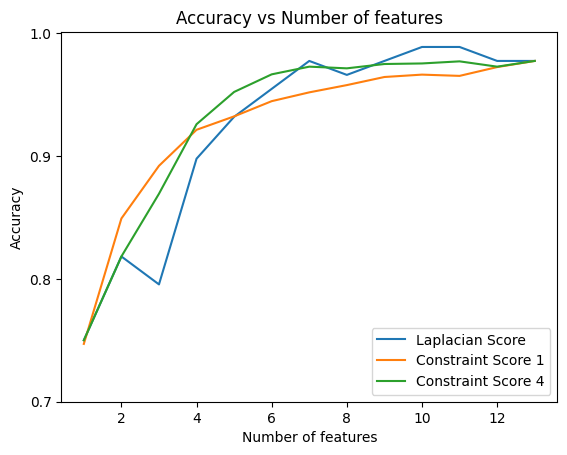
\includegraphics[height=0.8\textheight]{../Images/allscores3.png}
    \end{center}
\end{frame}

\begin{frame}{Results}

    \begin{center}
    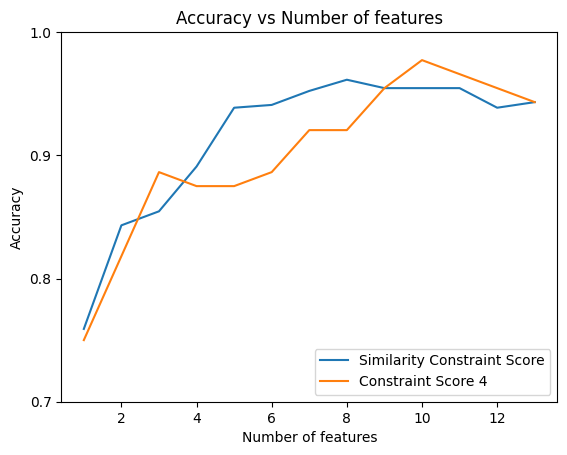
\includegraphics[height=0.8\textheight]{../Images/simCS.png}
    \end{center}
\end{frame}


\printbibliography

\end{document}